% !TEX root = ./article.tex

\documentclass{article}

\usepackage{mystyle}
\usepackage{myvars}



%-----------------------------

\begin{document}

	\maketitle % Insert title

	\thispagestyle{fancy} % All pages have headers and footers


%-----------------------------
%	ABSTRACT
%-----------------------------

	\begin{abstract}
		\noindent [TODO ]
	\end{abstract}

%-----------------------------
%	TEXT
%-----------------------------
	\section{Introducción}
	\label{sec:intro}

		\paragraph{}
		[TODO ]


	\section{Redes Bayesianas}
	\label{sec:bayes_network}

		\paragraph{}
		[TODO ]

		\subsection{Estructura Naive Bayes}
		\label{sec:structure_naive}

			\paragraph{}
			[TODO ]


		\subsection{Estructura TAN}
		\label{sec:structure_tan}

			\paragraph{}
			[TODO ]


		\subsection{Estructura K2}
		\label{sec:structure_K2}

			\paragraph{}
			[TODO ]



	\section{Experimentos}
	\label{sec:experiments}

		\paragraph{}
		[TODO ]

		\subsection{Conjuntos de Datos}

			\paragraph{}
			[TODO ]

			\begin{itemize}
				\item \textbf{Datos\_Credit\_100}: [TODO ]
				\item \textbf{Datos\_Credit\_1000}: [TODO ]
				\item \textbf{Datos\_Credit\_10000}: [TODO ]
				\item \textbf{Test\_Credit\_1000}: [TODO ]
			\end{itemize}


		\subsection{Resultados}

			\begin{figure}[h]
				\centering
				\begin{subfigure}{.32\textwidth}
					\centering
					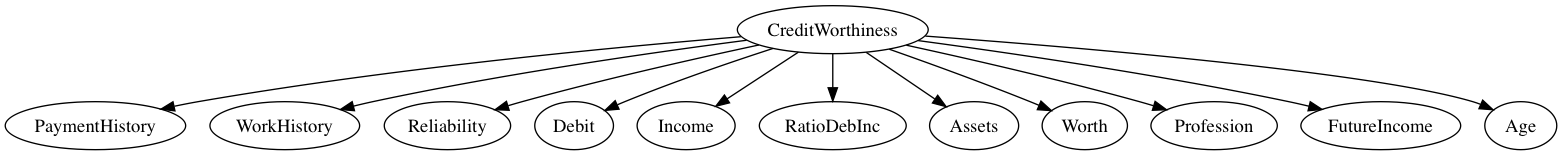
\includegraphics[width=\linewidth]{bayesnet-simple-100}
					\caption{Naive Bayes - 100}
				\end{subfigure} \
				\begin{subfigure}{.32\textwidth}
					\centering
					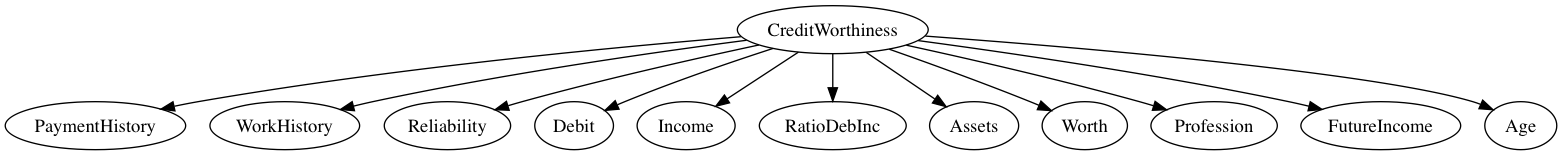
\includegraphics[width=\linewidth]{bayesnet-simple-1000}
					\caption{Naive Bayes - 1000}
				\end{subfigure} \
				\begin{subfigure}{.32\textwidth}
					\centering
					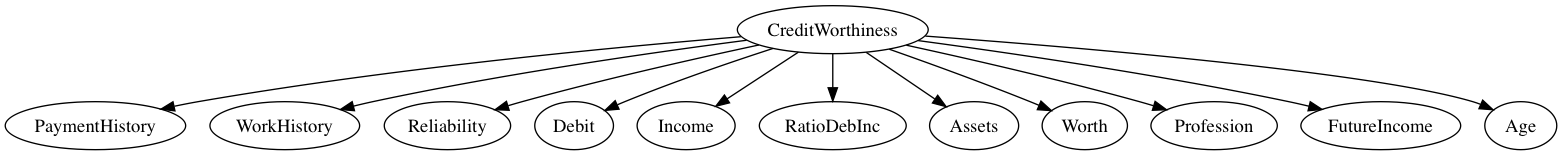
\includegraphics[width=\linewidth]{bayesnet-simple-10000}
					\caption{Naive Bayes - 10000}
				\end{subfigure} \\
				\begin{subfigure}{.32\textwidth}
					\centering
					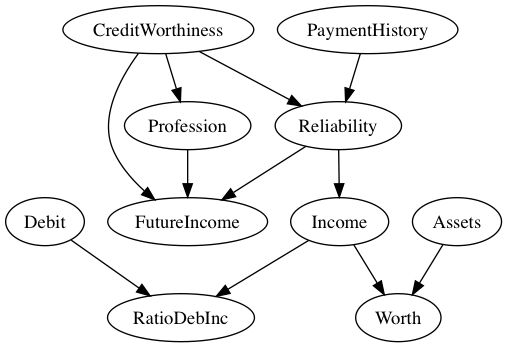
\includegraphics[width=\linewidth]{bayesnet-k2-100}
					\caption{K2 - 100}
				\end{subfigure} \
				\begin{subfigure}{.32\textwidth}
					\centering
					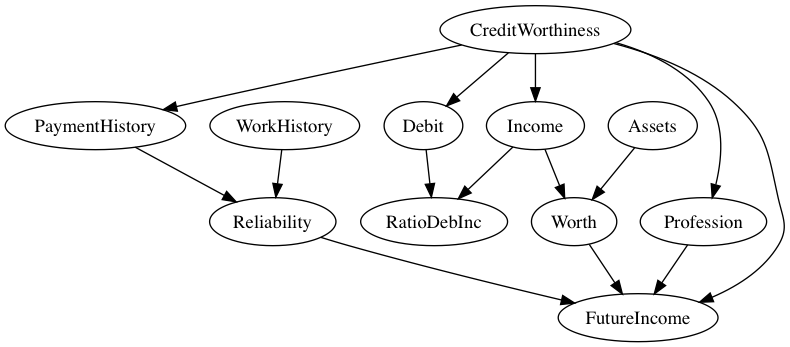
\includegraphics[width=\linewidth]{bayesnet-k2-1000}
					\caption{K2 - 1000}
				\end{subfigure} \
				\begin{subfigure}{.32\textwidth}
					\centering
					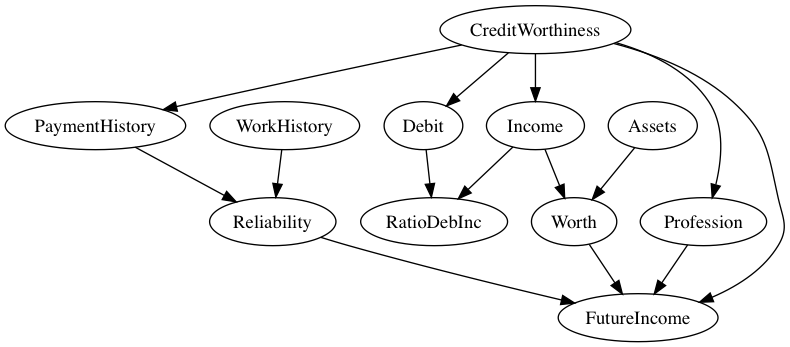
\includegraphics[width=\linewidth]{bayesnet-k2-1000}
					\caption{K2 - 10000}
				\end{subfigure} \\
				\begin{subfigure}{.32\textwidth}
					\centering
					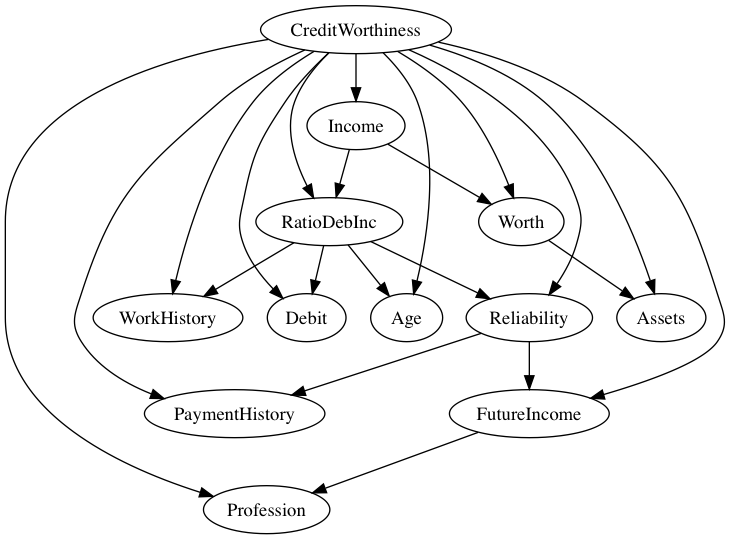
\includegraphics[width=\linewidth]{bayesnet-tan-100}
					\caption{TAN - 100}
				\end{subfigure} \
				\begin{subfigure}{.32\textwidth}
					\centering
					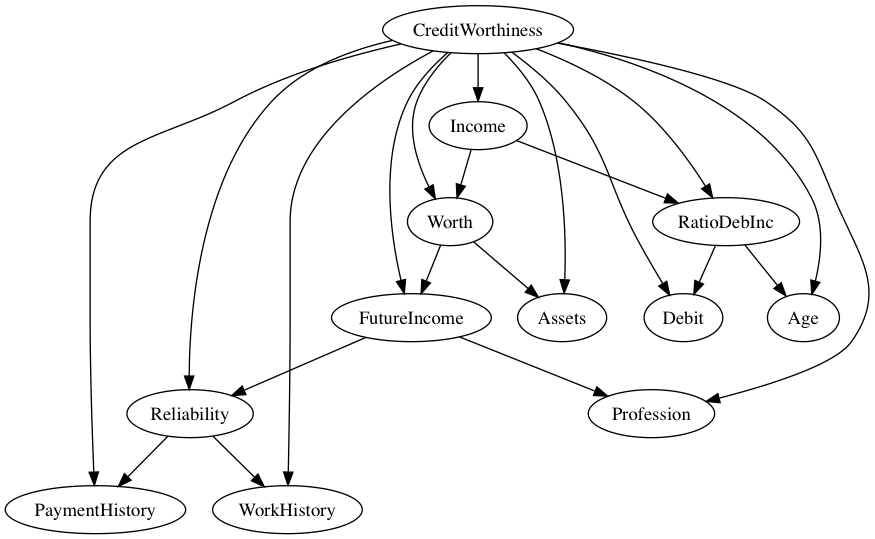
\includegraphics[width=\linewidth]{bayesnet-tan-1000}
					\caption{TAN - 1000}
				\end{subfigure} \
				\begin{subfigure}{.32\textwidth}
					\centering
					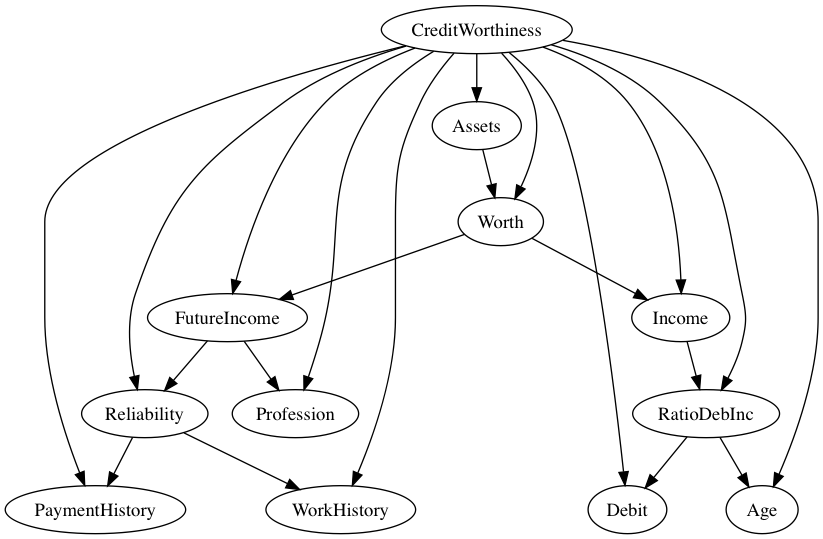
\includegraphics[width=\linewidth]{bayesnet-tan-10000}
					\caption{TAN - 10000}
				\end{subfigure}
				\caption{Redes Bayesianas generadas a partir de DatosCredit}
				\label{fig:bayes_network}
			\end{figure}


			\paragraph{}
			[TODO ]
%-----------------------------
%	Bibliographic references
%-----------------------------
	\nocite{garciparedes:machine-learning-bayesian-2}
	\nocite{subject:taa}
	\nocite{tool:weka}
  \bibliographystyle{alpha}
  \bibliography{bib/misc}

\end{document}
